\section{Theory}
A capacitor stores electric charge using two conducting plates separated by a dielectric material. A reverse-biased p-n junction diode has p-type and n-type regions acting as the capacitor's electrodes, while the depletion region acts as the dielectric. Hence, the diode acts as a parallel plate capacitor, with its capacitance changing as the applied voltage changes. Increasing the reverse bias voltage moves the majority carriers away from the p-n junction, widening the depletion region and reducing the size of the p-type and n-type regions.

The p-n junction capacitance is given by,
\begin{equation}
    C=\frac{dQ}{dV_{dc}}=\frac{\epsilon_o \epsilon_s A}{x_d}
    \label{eq:1}
\end{equation}
where Q is the charge, $V_{DC}$ is the reverse bias voltage applied, $\epsilon_0$ is the permittivity of empty space, $\epsilon_s$ is the semiconductor's dielectric constant, and A is the area of the p-n junction. In a reverse biassed junction with constant doping density $N_d$, the depletion area width is determined by,
\begin{equation}
    x_d=\sqrt{\frac{2 \epsilon_o \epsilon_s (V_{bi}+V_{dc})}{qN_d}}
    \label{eq:2}
\end{equation}
$V_{bi}$ is the built-in voltage,$V_{dc}$ is the reverse voltage, and q is the charge of an electron. From equations (1) and (2), we have,
\begin{equation}
    \frac{1}{C^2}=\left(\frac{x_d}{\epsilon_o \epsilon_s A}\right)^2=\frac{2 (V_{bi}+V_{dc})}{q N_d \epsilon_o \epsilon_s A^2}
    \label{eq:3}
\end{equation}
By plotting $\frac{1}{C^2}$ versus $V_{DC}$, doping density and built-in potential can be determined.

In commercially available diodes, the
junction capacitance is designed to be as low as possible to
enable fast switching operation. This poses problems in the
measurement of capacitance of such devices in the laboratory using educational grade measurement equipment. To
overcome this limitation, we use a solar cell, which is essentially a large area p-n junction diode that thereby has larger
and hence measurable capacitance.
% ======================================================================================
\section{Experimental Setup}

\subsection*{Apparatus}

\begin{enumerate}
    \item Solar cell
    \item Resistors of 1k$\Omega$ and 10k$\Omega$
    \item IC 741 opamps
    \item DC power supply
    \item Function Generator 
    \item Connecting wires\\
\end{enumerate}

The circuit shown in Fig. \ref{th:1} can measure the capacitance of a p-n junction device, such as a solar cell. The capacitance of the device depends on the applied DC voltage. To measure the C-V profile, the circuit applies a variable DC bias and a small AC signal to the solar cell. The circuit uses an inverting summing amplifier that adds the variable DC voltage (with unity gain $R/R_2$) and the small signal AC voltage (with attenuation factor 1/10 = $R/R_1$). The output voltage of the amplifier is connected to the solar cell. The AC signal is small enough not to perturb the DC bias or affect the charge polarization due to the DC bias. The voltage $V_{DUT}$ in Fig. \ref{th:1} is thus given by the following equation:
	\begin{equation}
		V_{DUT}=-R\left(\frac{V_{DC}}{R_2}+\frac{V_{AC}}{R_1}\right)
		\label{eq:4}
	\end{equation}

	\begin{figure}
		\centering
		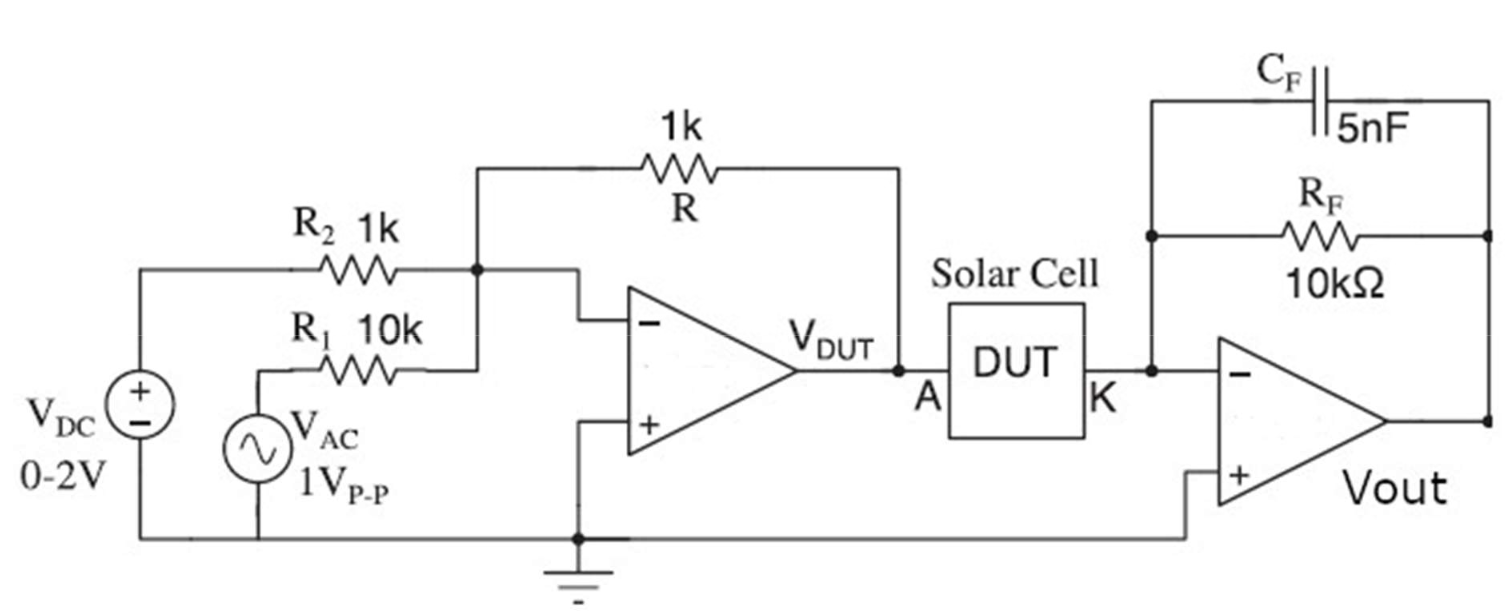
\includegraphics[width=1\columnwidth]{images/circuit.png}
		\caption{Circuit for experimental setup}
		\label{th:1}
	\end{figure}

In our experiment, the AC voltage across the solar cell is set to be one-tenth of the input DC voltage, due to instrument sensitivity limitations. The summing circuit connects the solar cell's anode (A) to its output, while negative feedback grounds the cathode (K). The capacitor's current is proportional to the applied AC sinusoidal voltage, and an I to V converter (trans-impedance amplifier) is used to convert this current into a voltage reading on a multimeter. The trans-impedance amplifier generates a voltage output that is proportional to the capacitance of the solar cell ($C_{DUT}$) and $V_{DUT}$. The following equation gives the magnitude of the AC component of the output voltage: 
\begin{equation}
    V_{OUT}=V_{DUT}\frac{C_{DUT}}{C_F}\frac{1}{\sqrt{1+\frac{1}{(\omega R_F C_F)^2}}}
    \label{eq:5}
\end{equation}
In our setup, we use the function generator to apply an AC voltage of 5 kHz. Since operational amplifiers exhibit $1/f$ noise at low frequencies (0.1 to 10 Hz), and this noise can go up to 2 kHz for fast operational amplifiers, we limit our frequency range to high frequencies. We use 741 opamps instead of TL071 opamps, and the circuit is shown in \hyperref[th:1]{Figure 1}. By varying the DC voltage in steps from 0 to 1.5 V using a DC power supply, we record $V_{OUT}$ (AC) and $V_{DUT}$ using different multimeters. We calculate $C_{DUT}$ using \hyperref[eq:4]{Equation 4}.